\documentclass{report}
\usepackage{amsfonts}
\usepackage{amsthm}
\usepackage{amsmath}
\usepackage{algorithmic}
\usepackage{algorithm}
\newtheorem{theorem}{Theorem}
\DeclareMathOperator{\trans}{trans}
\addtolength{\parskip}{3mm}
\title{\Huge\sc True Facts}
\author{Al Caveman}
\usepackage{graphicx}
\usepackage{eso-pic}
\newcommand\BackgroundPic{
\put(-5,-190){
\parbox[b][\paperheight]{\paperwidth}{%
\vfill
\centering
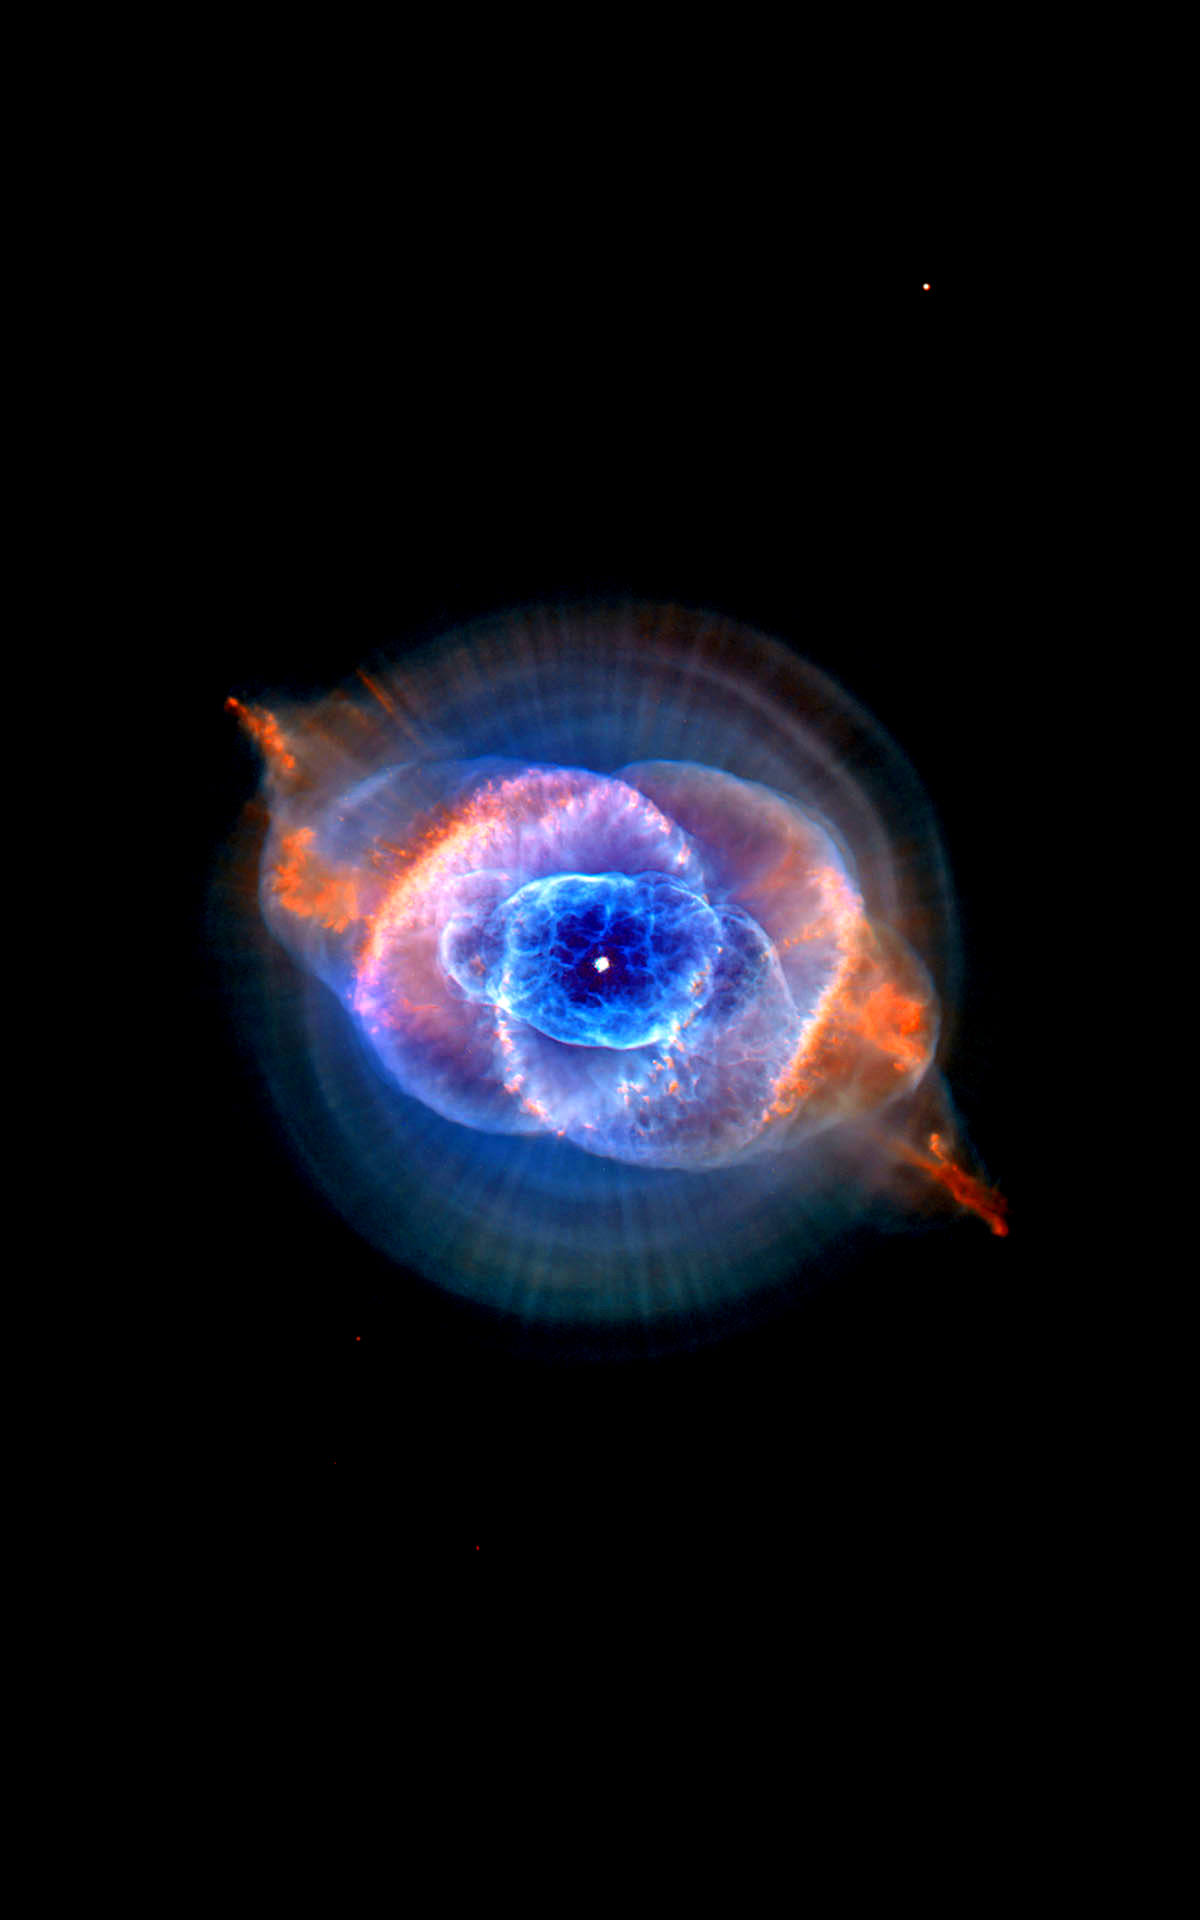
\includegraphics[width=1.01\paperwidth, keepaspectratio]{background.png}%
\vfill
}}}
\begin{document}
\AddToShipoutPicture*{\BackgroundPic}
\begin{titlepage}
\centering
\color{white}{{\Huge\sc True Facts}\\\vspace{1cm}\Large Al Caveman\\\vspace{0.5cm}2015}
\end{titlepage}

\chapter*{Preface}
This book's primary objective is to educate you about difficult/non-obvious
(but nonetheless important) facts about the universe that you live in. This
book is written with the spirit that you, monkeys, are able to learn.  This
book is also highly anticipated:
\begin{quote}
``\textbf{Al-Caveman:} RobbieAB$|$work, would u read my book?
\textbf{RobbieAB$|$work:} Depends how bored I am.
\textbf{Al-Caveman:} ok. i take that as \emph{yes}.'' ---
Freenode/\#gentoo-chat-exile, 2015
\end{quote}

\begin{quote}
``\textbf{Al-Caveman:} DistantStar, u?
\textbf{DistantStar:} okay.
\textbf{Al-Caveman:} perfect.'' --- Freenode/\#gentoo-chat-exile, 2015
\end{quote}

\tableofcontents

\chapter{History}
\section{The Past}
There are multiple possible reasons why you exist, but the one that is easiest
to explain by monkeys like you (which is not necessarily the true one) is one
that tries to minimize the role of miracles/magic. Turns out that your fellow
monkeys found one that they think it minimizes that, and they decided to call
it ``\emph{evolution}'', and it looks exactly like this:
\begin{algorithm}
\caption{The algorithm that made you.}
\label{alg:evolv}
\begin{algorithmic}
    \FOR{1 ... $t$}
        \STATE{$\trans(\mathcal{U})$}
    \ENDFOR
\end{algorithmic}
\end{algorithm}

Where $t$ is the total number of clock ticks, $\mathcal{U}$ is the set of all
elements of the universe, and $\trans$ is a function that randomly transforms
elements in $\mathcal{U}$ based on some distribution that I'll touch later. For
any $\bf{x} \in \mathcal{U}$, $\bf{x}$ is a vector whose components describe
exactly the perfect state of element $x$. You are $\mathcal{M}$ for monkey,
where $\mathcal{M} \subset \mathcal{U}$.

The reason you exist is because Allah\footnote{This material is not
religion-oriented. Feel free to put your favorite God there including
\emph{none}.} decided to execute Algorithm \ref{alg:evolv} such that $t$ is a
large enough number, and the distribution that the function $\trans$
adheres to is a special one that permits your kind to exist.

No monkey (or group of monkeys) is known to fully know the distribution that
$\trans$ tries to maintain, but some have figured out a few consistent
rules that this distribution seems to stick to, which the monkeys decided to
call ``\emph{Laws of Physics}''.

For example, imagine some particular state of the universe (i.e. a point in
time where the vectors in $\mathcal{U}$ have particular values) where there is an apple
atop the surface of planet earth by a few meters. In this particular
configuration, the function $\trans$ will modify the values of elements of
$\mathcal{U}$ as the clock advances such that the apple and earth will achieve a shorter
euclidean distance between them until they hit each other. Once they hit each
other, then other consistent patterns happen that the monkeys have figured out.

Hundreds of years ago, monkeys were thinking/conjecturing that
this distribution is fully deterministic. I.e. the way $\trans$ will
transform the elements in $\mathcal{U}$ in the future (i.e. next clock tick) is fully
dependant on the current values in $\mathcal{U}$ at the present time (i.e. current clock
tick).

Later on, some other monkeys (that stood on the shoulders of previous giant
monkeys), suggested that there might be some intrinsic randomness inside the
function $\trans$ that we can never fully know. At that time, some yet
other monkeys didn't like this idea and said things like ``\emph{God doesn't
play dice}''.

But before we answer whether the function $\trans$ has an intrinsic
randomness that no one can predict (i.e. beyond the information in $\mathcal{U}$ of a
previous time), we need to know what is randomness? Do you know any algorithm
that perfectly tells you if a number sequence is random for everyone (i.e.
universally random and not relevant to the observer)?\footnote{A monkey named
\textbf{\_anomaly\_} in Freenode's \#gentoo-chat-exile claimed ``\emph{yes}'',
but then he retreated as he failed to find an algorithm that does that. He then
claimed that he is not a mathematician. But somehow he dares to make claims
about mathematics.}.

\section{The Present}
The specific configuration of elements in $\mathcal{U}$ at some point in time between 1
and $t$ as configured by Algorithm \ref{alg:evolv}. I am pretty sure it's not 1,
and I feel (at the time of writing this) that it's not $t$ either. I can
confirm now that it wasn't $t$ back then.

\section{The Future}
The specific configuration of elements in $\mathcal{U}$ as configured by Algorithm
\ref{alg:evolv} when the clock tick is a number that is greater than the number
of the clock tick of some reference point that you consider the
``\emph{present}''. Many monkeys call this the ``\emph{future}''.

\chapter{Good and Bad}

\end{document}
